\documentclass[aspectratio=169,10pt]{beamer}
\hfuzz=12pt
\vfuzz=14pt

\usetheme{metropolis}
\metroset{block=fill, sectionpage=progressbar, numbering=fraction}

\usepackage{amsmath,amssymb}
\usepackage{tikz}
\usetikzlibrary{arrows.meta,positioning,calc}
\usepackage{array,booktabs}
\usepackage{xcolor}

\definecolor{giublue}{RGB}{30,58,138}
\definecolor{giuaccent}{RGB}{13,148,136}
\setbeamercolor{frametitle}{bg=giublue}
\setbeamercolor{progress bar}{fg=giuaccent}
\setbeamercolor{alerted text}{fg=giuaccent}
\setbeamerfont{title}{size=\large}
\setbeamerfont{subtitle}{size=\scriptsize}
\setbeamerfont{institute}{size=\scriptsize}
\setbeamerfont{date}{size=\tiny}

\title{Reinforcement Learning for Simple Adaptive Robot Behavior}
\subtitle{Topic 6 / Track 8 --- Learning, Personalization \& Adaptation in HRI}
\author{Nour Gaser \and Eman Saleh}
\institute{German International University (GIU) \\ Interactive \& Social AI for Humanoid Robots}
\date{Draft --- \today}

\newcommand{\E}{\mathbb{E}}
\newcommand{\refnum}[1]{{\footnotesize\color{giuaccent}[#1]}}

\hypersetup{pdftitle={Reinforcement Learning for Simple Adaptive Robot Behavior}, pdfauthor={Nour Gaser and Eman Saleh}, pdfkeywords={HRI, reinforcement learning, personalization, adaptation, NAO}}
\pdfstringdefDisableCommands{\def\translate#1{#1}}

\begin{document}

\maketitle

\begin{frame}{Roadmap}
  \tableofcontents
\end{frame}

\section{Framing \& Foundations}

\begin{frame}{What this topic is --- and where it sits}
  \textbf{Our assigned topic:} \alert{Reinforcement Learning for Simple Adaptive Robot Behavior.}
  \vspace{0.6em}
  \begin{itemize}
    \item Realized through \textbf{Topic 6: Learning in HRI} (RL vs.\ SL, learning from demonstration, personalization).
    \item Anchored in the seminar's \textbf{Track 8: Personalization \& Adaptation} paper set.
    \item Implemented under \textbf{Project Track D: Adaptive \& Learning Systems} on the \textbf{NAO} robot.
  \end{itemize}
  \vspace{0.6em}
  \begin{block}{The one-sentence thesis}
    A robot can \emph{learn online}, from a person's social signals as a \emph{reward}, to adapt simple social behaviors --- formalized as a Markov Decision Process and solved with lightweight RL.
  \end{block}
\end{frame}

\begin{frame}{Robots, social robots, and HRI}
  \begin{columns}[T]
    \begin{column}{0.50\textwidth}
      \textbf{Robot:} an embodied machine that \emph{senses}, \emph{computes}, and \emph{acts} on the world.

      \medskip
      \textbf{Social robot:} interacts with people following social rules, using human-like cues.

      \medskip
      \textbf{HRI:} the interdisciplinary field --- robotics, AI, psychology, design --- studying how people and robots interact.
    \end{column}
    \begin{column}{0.44\textwidth}
      \textbf{Core challenges}
      \begin{itemize}
        \item Embodiment --- the body shapes interaction
        \item Autonomy --- how much the robot decides
        \item Trust --- whether people rely on it
      \end{itemize}
      \medskip
      \textbf{Modalities \& signals}
      \begin{itemize}
        \item Speech, gesture, gaze, \alert{proxemics} (space)
        \item \alert{Social signals} (gaze, repositioning, touch) $\rightarrow$ our \emph{reward}
      \end{itemize}
    \end{column}
  \end{columns}
\end{frame}

\section{Learning Paradigms}

\begin{frame}{Three ways a machine can learn}
  \begin{columns}[T]
    \begin{column}{0.33\textwidth}
      \textbf{Supervised}
      \begin{itemize}\footnotesize
        \item Learn input $\to$ correct label from examples.
        \item Needs large \emph{pre-labeled} data; trained \emph{offline}.
        \item E.g.\ emotion classifier from labeled images.
      \end{itemize}
    \end{column}
    \begin{column}{0.33\textwidth}
      \textbf{Unsupervised}
      \begin{itemize}\footnotesize
        \item Find structure in \emph{unlabeled} data.
        \item Clustering, dimensionality reduction.
        \item E.g.\ group users by interaction style.
      \end{itemize}
    \end{column}
    \begin{column}{0.33\textwidth}
      \textbf{\alert{Reinforcement}}
      \begin{itemize}\footnotesize
        \item Learn by \emph{trial and error} from a \emph{reward}.
        \item No labels; adapts \emph{online}.
        \item E.g.\ adjust distance if the person leans in / backs away.
      \end{itemize}
    \end{column}
  \end{columns}
  \vspace{0.8em}
  \begin{alertblock}{Why not just supervised learning?}
    The ``correct'' social behavior is person- and context-specific, unknown in advance, and shifts \emph{during} interaction. Supervised learning needs a labeled answer up front and cannot adapt mid-interaction. RL learns the answer \emph{from} the interaction.
  \end{alertblock}
\end{frame}

\section{Reinforcement Learning in Depth}

\begin{frame}{The RL loop: agent, environment, reward}
  \begin{columns}[c,onlytextwidth]
    \begin{column}{0.42\textwidth}
      \centering
      \resizebox{\linewidth}{!}{%
      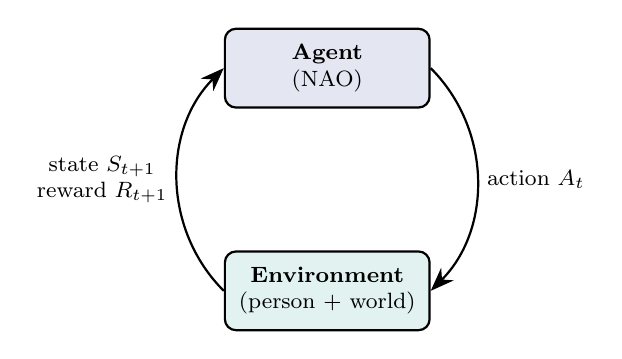
\begin{tikzpicture}[
        node distance=1.4cm,
        box/.style={draw, rounded corners, minimum width=2.6cm, minimum height=1cm, align=center, thick},
        every node/.style={font=\footnotesize}]
        \node[box, fill=giublue!12] (agent) {\textbf{Agent}\\(NAO)};
        \node[box, fill=giuaccent!12, below=1.8cm of agent] (env) {\textbf{Environment}\\(person + world)};
        \draw[-{Stealth[length=3mm]}, thick]
          (agent.east) to[bend left=45] node[right, midway]{action $A_t$} (env.east);
        \draw[-{Stealth[length=3mm]}, thick]
          (env.west) to[bend left=45] node[left, midway, align=center]{state $S_{t+1}$\\reward $R_{t+1}$} (agent.west);
      \end{tikzpicture}%
      }
    \end{column}
    \begin{column}{0.50\textwidth}
      At each step $t$ the agent:
      \begin{enumerate}\footnotesize
        \item observes state $S_t$,
        \item takes action $A_t$ via policy $\pi(a\mid s)$,
        \item receives reward $R_{t+1}$,
        \item lands in state $S_{t+1}$.
      \end{enumerate}
      \medskip
      \textbf{Goal:} find $\pi$ maximizing expected \emph{discounted return}
      \[
        G_t=\textstyle\sum_{k\ge 0}\gamma^{k}R_{t+k+1},\quad \gamma\in[0,1).
      \]
      \textbf{Value} $Q(s,a)$ = expected return from taking $a$ in $s$.
    \end{column}
  \end{columns}
  \vfill
  {\footnotesize\raggedright Formalized as an MDP $\langle S,A,P,R,\gamma\rangle$: the next state depends only on current $(s,a)$ --- the \emph{Markov property}. \refnum{Sutton2018}\par}
\end{frame}

\begin{frame}{Q-learning: the workhorse for \emph{simple} adaptive behavior}
  \textbf{Idea:} learn the value of each (state, action) pair directly --- no model of the world needed.
  \vspace{0.4em}
  \begin{block}{Q-learning update (Watkins \& Dayan, 1992)}
    \[
      Q(s,a)\;\leftarrow\;Q(s,a)\;+\;\alpha\Big[\,\underbrace{r+\gamma\max_{a'}Q(s',a')}_{\text{target}}\;-\;Q(s,a)\,\Big]
    \]
    \footnotesize $\alpha$: learning rate \quad $\gamma$: discount \quad $r$: observed reward
  \end{block}
  \vspace{0.2em}
  \begin{columns}[T]
    \begin{column}{0.5\textwidth}
      \textbf{Exploration vs.\ exploitation}
      \begin{itemize}\footnotesize
        \item Must try new actions \emph{and} use known-good ones.
        \item \alert{$\varepsilon$-greedy}: random action w.p.\ $\varepsilon$, else $\arg\max_a Q(s,a)$; decay $\varepsilon$ over time.
      \end{itemize}
    \end{column}
    \begin{column}{0.5\textwidth}
      \textbf{Tabular vs.\ approximation}
      \begin{itemize}\footnotesize
        \item \emph{Tabular}: one value per $(s,a)$ --- perfect for small, discrete spaces (our case).
        \item Large/continuous $\to$ function approximation (Deep Q-Networks).
      \end{itemize}
    \end{column}
  \end{columns}
\end{frame}

\begin{frame}{Policy gradients \& learning from \emph{human} reward}
  \begin{columns}[T]
    \begin{column}{0.5\textwidth}
      \textbf{Policy gradient (REINFORCE)}
      \begin{itemize}\footnotesize
        \item Directly tune a parameterized policy $\pi_\theta$ toward higher reward.
        \item Natural fit for \emph{continuous} action parameters: distance, speed, timing.
        \item Used by Mitsunaga et al.\ to adapt proxemics, gaze \& timing on a social robot. \refnum{Mitsunaga2005}
      \end{itemize}
    \end{column}
    \begin{column}{0.5\textwidth}
      \textbf{Interactive RL / human feedback}
      \begin{itemize}\footnotesize
        \item The \emph{human} supplies the reward signal.
        \item \alert{TAMER}: non-experts shape an agent via approval / disapproval. \refnum{Knox2009}
        \item Cuts the number of trials needed --- crucial on hardware.
      \end{itemize}
    \end{column}
  \end{columns}
  \vspace{0.6em}
  \begin{alertblock}{The hardware reality (a recurring theme)}
    Every real trial costs \emph{time}, \emph{battery}, and \emph{joint wear}. So \textbf{sample efficiency} matters, and \textbf{sim-to-real transfer} (the ``reality gap'') is a genuine risk: policies that work in simulation can fail on the physical robot.
  \end{alertblock}
\end{frame}

\begin{frame}{Learning from Demonstration (LfD) --- a complement to RL}
  \begin{columns}[T]
    \begin{column}{0.55\textwidth}
      \textbf{Teach by showing}, not by coding or rewarding. \refnum{Argall2009}
      \begin{itemize}
        \item Intuitive for non-experts --- people teach by demonstrating.
        \item \alert{Kinesthetic teaching}: set joint stiffness to zero, physically move NAO's limb, record the joint trajectory, replay it.
      \end{itemize}
    \end{column}
    \begin{column}{0.43\textwidth}
      \begin{block}{Why pair LfD with RL?}
        A demonstration gives a good \emph{starting policy}; RL then \emph{refines} it through interaction --- fixing RL's slow cold-start and poor sample efficiency.
      \end{block}
    \end{column}
  \end{columns}
\end{frame}

\section{Personalization \& Adaptation}

\begin{frame}{Personalization in long-term HRI}
  \begin{columns}[T]
    \begin{column}{0.56\textwidth}
      \textbf{Why adapt at all?}
      \begin{itemize}\footnotesize
        \item Short-term studies hide the hard part: sustaining engagement over many sessions. \refnum{Irfan2019}
        \item Adaptation counters the \alert{novelty effect} --- interest fades once a robot stops being new.
        \item Built on \emph{user modeling} + \emph{incremental / lifelong learning}. \refnum{Irfan2021}
      \end{itemize}
    \end{column}
    \begin{column}{0.42\textwidth}
      \textbf{Static vs.\ dynamic}
      \begin{itemize}\footnotesize
        \item \emph{Static}: fix a profile once (a questionnaire).
        \item \alert{Dynamic}: adjust in real time to live social signals --- our RL approach.
      \end{itemize}
    \end{column}
  \end{columns}
  \vspace{0.6em}
  \begin{alertblock}{The ethical edge: entertainment vs.\ manipulation \refnum{Pollmann2023}}
    The same personalization that improves user experience can be used to \emph{steer} a person against their own autonomy. Adaptive systems need explicit ethical guardrails --- a point we will state up front, not bolt on.
  \end{alertblock}
\end{frame}

\section{Literature Review}

\begin{frame}{Anchor papers (Track 8 set)}
  \begin{itemize}
    \item \textbf{Irfan et al.\ (2019), \emph{Personalization in Long-Term HRI}.} Establishes the premise: adaptation/personalization are \emph{necessary} to sustain engagement and build trust. \refnum{Irfan2019}
    \item \textbf{Irfan et al.\ (2021), \emph{Lifelong Learning \& Personalization (LEAP-HRI)}.} Robots ``in the wild'' must learn new concepts incrementally without forgetting. \refnum{Irfan2021}
    \item \textbf{Tozadore et al.\ (2018), \emph{Towards Adaptation \& Personalization in Task-Based HRI}.} A concrete personalization framework on a humanoid; classifies user signals to adapt activities and prolong interaction. \refnum{Tozadore2018}
    \item \textbf{Pollmann et al.\ (2023), \emph{Entertainment vs.\ Manipulation}.} User-centered + ethical analysis of a personalized robot; personalization helps UX but risks manipulation. \refnum{Pollmann2023}
  \end{itemize}
\end{frame}

\begin{frame}{Added papers --- the RL ``how'' the anchors leave open}
  \begin{itemize}
    \item \textbf{Mitsunaga et al.\ (2005/2008), \emph{Robot Behavior Adaptation via Policy-Gradient RL}.} The seminal method: a social robot uses policy-gradient RL to adjust \emph{interaction distance, gaze meeting, and motion speed/timing}, reading subconscious human comfort signals as reward; adapts to individual preferences across 12 subjects. \refnum{Mitsunaga2005}
    \item \textbf{Patompak et al.\ (2020), \emph{Learning Proxemics for Personalized HRI}.} Builds a Social Force Model via fuzzy inference and tunes it with RL so the robot learns each person's comfortable interaction distance; validated in simulation and on a real robot. \refnum{Patompak2020}
  \end{itemize}
  \vspace{0.4em}
  {\footnotesize \emph{Rationale:} the anchors explain \emph{why} and \emph{what} to personalize; these two supply concrete \emph{RL mechanisms} for adapting social behavior --- with the proxemics formulation that maps cleanly onto NAO's sonar + tactile sensors.}
\end{frame}

\begin{frame}{Methodological critique \& research gaps}
  \begin{itemize}
    \item \textbf{Reality gap:} fast convergence in simulation, but sensor noise and dynamics differ on hardware.
    \item \textbf{Sample efficiency:} real trials are slow and cause wear --- few-shot learning, human reward, and LfD warm-starts help.
    \item \textbf{Reward specification:} ``social reward'' is noisy and hard to define; bad rewards yield awkward behavior.
    \item \textbf{Static vs.\ dynamic preference:} treating preference as fixed fails long-term.
    \item \textbf{Evaluation:} over-reliance on subjective post-hoc surveys; need to \emph{combine} objective sensor metrics with subjective scales.
    \item \textbf{Generalization \& reproducibility:} per-user policies may not transfer; HRI lacks standardized metrics/protocols.
  \end{itemize}
  \begin{block}{}
    \footnotesize These gaps are our \textbf{Q\&A defense} --- for each we will hold a one-line position grounded in the literature.
  \end{block}
\end{frame}

\section{The NAO Platform}

\begin{frame}{NAO V6 --- our research platform}
  \begin{columns}[T]
    \begin{column}{0.5\textwidth}
      \textbf{Hardware} \refnum{Aldebaran}
      \begin{itemize}\footnotesize
        \item 58\,cm, $\sim$5.6\,kg, \textbf{25 degrees of freedom}
        \item Dual 5\,MP cameras; 4 microphones (sound localization)
        \item \alert{Sonar} distance sensors: $\sim$25--255\,cm
        \item \alert{Tactile} sensors (head + hands); foot force sensors; IMU; joint encoders
        \item Battery: \textbf{45--90\,min}; limited onboard compute
      \end{itemize}
    \end{column}
    \begin{column}{0.5\textwidth}
      \textbf{Software (NAOqi SDK)}
      \begin{itemize}\footnotesize
        \item \texttt{ALMotion} --- joints, posture, stiffness, walking
        \item \texttt{ALMemory} / \texttt{ALSensors} --- sensor blackboard
        \item \texttt{ALSonar} --- distance; \texttt{ALTextToSpeech} --- speech
        \item \textbf{Choregraphe} IDE (with a \emph{virtual} NAO)
        \item Python / C++ SDKs; ROS support
      \end{itemize}
    \end{column}
  \end{columns}
  \vspace{0.4em}
  \begin{alertblock}{Open question for the instructors}
    Which NAO version is on campus, and may we run trials on the physical robot? Until confirmed, we prototype the full RL loop in \textbf{simulation / mocked NAOqi}.
  \end{alertblock}
\end{frame}

\section{Project Pitch}

\begin{frame}{Three candidate experiments (all NAO + RL, 2-person, 2--4 weeks)}
  \footnotesize
  \begin{table}
    \begin{tabular}{@{}>{\raggedright\arraybackslash}p{2.4cm}>{\raggedright\arraybackslash}p{3.1cm}>{\raggedright\arraybackslash}p{3.0cm}>{\raggedright\arraybackslash}p{2.6cm}@{}}
      \toprule
      \textbf{Option} & \textbf{Adaptive behavior} & \textbf{Reward signal} & \textbf{Baseline} \\
      \midrule
      \textbf{(A)} Greeting / social distance & Approach distance + greeting intensity & Tactile ``approve'' + sonar distance change & Fixed scripted greeting \\
      \addlinespace
      \textbf{(B)} Tutoring / pace & Speech rate, pauses, difficulty & Answer correctness + engagement & Fixed-pace tutor \\
      \addlinespace
      \textbf{(C)} Engagement max. & Pick from behavior repertoire (joke, gesture, question) & Change in gaze + proximity & Random / fixed rotation \\
      \bottomrule
    \end{tabular}
  \end{table}
  \vspace{0.4em}
  All three are deliberately kept \textbf{open}. They share one RL loop --- only the state, actions, and reward wiring differ. \alert{We are not pre-committing}: we would like the discussion to pick a direction (from these, or a new one you suggest).
\end{frame}

\begin{frame}{Shared architecture --- why any direction is one line away}
  \footnotesize
  Every candidate experiment uses the \emph{same} RL loop; only the state/action/reward bindings change. An abstract robot interface lets the identical loop run on laptop, simulator, or real NAO.
  \vspace{0.15em}
  \begin{columns}[c,onlytextwidth]
    \begin{column}{0.46\textwidth}
      \centering
      \resizebox{\linewidth}{!}{%
      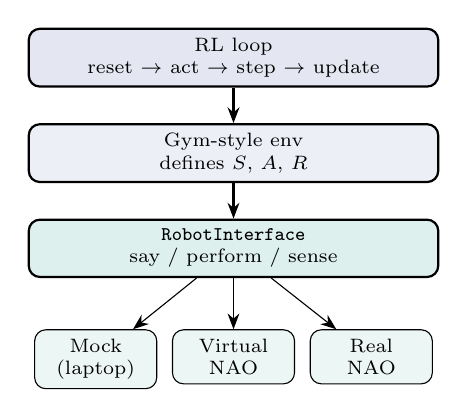
\begin{tikzpicture}[
        node distance=0.45cm,
        layer/.style={draw, rounded corners, minimum width=5.2cm, minimum height=0.68cm, align=center, thick, font=\scriptsize},
        impl/.style={draw, rounded corners, minimum width=1.55cm, minimum height=0.62cm, align=center, font=\scriptsize}]
        \node[layer, fill=giublue!12] (loop) {RL loop \\ {\scriptsize reset $\to$ act $\to$ step $\to$ update}};
        \node[layer, fill=giublue!8, below=of loop] (env) {Gym-style env \\ {\scriptsize defines $S$, $A$, $R$}};
        \node[layer, fill=giuaccent!14, below=of env] (iface) {\texttt{RobotInterface} \\ {\scriptsize say / perform / sense}};
        \node[impl, fill=giuaccent!8, below=0.65cm of iface, xshift=-1.75cm] (mock) {Mock \\ (laptop)};
        \node[impl, fill=giuaccent!8, below=0.65cm of iface] (sim) {Virtual \\ NAO};
        \node[impl, fill=giuaccent!8, below=0.65cm of iface, xshift=1.75cm] (real) {Real \\ NAO};
        \draw[-{Stealth[length=2mm]}, thick] (loop)--(env);
        \draw[-{Stealth[length=2mm]}, thick] (env)--(iface);
        \draw[-{Stealth[length=2mm]}] (iface)--(mock);
        \draw[-{Stealth[length=2mm]}] (iface)--(sim);
        \draw[-{Stealth[length=2mm]}] (iface)--(real);
      \end{tikzpicture}%
      }
    \end{column}
    \begin{column}{0.50\textwidth}
      \begin{itemize}\footnotesize
        \item \textbf{Already built \& running} on the laptop mock --- this is our ``implementation has begun''.
        \item \alert{Sensor noise injected} in the mock to harden the policy and shrink the eventual reality gap.
        \item Swapping to a NAO is literally:
      \end{itemize}
      \vspace{0.05em}
      {\scriptsize\ttfamily
      \textcolor{gray}{\# robot = MockRobot()}\\
      robot = NaoRobot(ip=...)\\
      }
      {\footnotesize \quad --- env and agent code unchanged.}
    \end{column}
  \end{columns}
\end{frame}

\begin{frame}[fragile]{Common NAOqi plumbing (excerpt of working code)}
  \scriptsize
  The seam that makes the swap trivial. The mock contains a simulated person so the loop runs with \emph{no hardware and no NAOqi SDK} today.
\begin{semiverbatim}\scriptsize
class RobotInterface(ABC):           \textcolor{gray}{# shared by mock / sim / real}
    def perform(self, action): ...   \textcolor{gray}{# 'closer','back','intensity_up'...}
    def sense(self) -> Signals: ...  \textcolor{gray}{# {distance, touch, present}}

class MockRobot(RobotInterface):     \textcolor{gray}{# laptop + hidden person model}
    def sense(self):
        return Signals(distance=self._d + noise,
                       touch=self._person_approves(),
                       present=self._present)

class NaoRobot(RobotInterface):      \textcolor{gray}{# real NAO via NAOqi}
    def sense(self):
        d = self.memory.getData(".../US/Left/Sensor/Value")
        touch = self.memory.getData("FrontTactilTouched") > 0.5
        \textcolor{gray}{# ... ALSonar + tactile + ALFaceDetection}
\end{semiverbatim}
  \vspace{-0.2em}
  \alert{Result so far:} on the illustrative greeting task, the learned policy beats a scripted baseline by $\sim +9$ reward, discovering ``don't crowd; settle in the personal zone'' from touch signals alone --- hosted on GitHub.
\end{frame}

\begin{frame}{Worked example (illustrative) --- a greeting MDP}
  {\footnotesize\emph{Not our chosen experiment} --- an illustration of how \emph{any} direction becomes a concrete MDP. This is the one we already implemented to validate the architecture.}
  \vspace{0.3em}
  \begin{columns}[T]
    \begin{column}{0.5\textwidth}
      \textbf{State $S$} (discretized)
      \begin{itemize}\footnotesize
        \item Distance bin: intimate / personal / social (from sonar)
        \item Current greeting intensity level
      \end{itemize}
      \textbf{Action $A$}
      \begin{itemize}\footnotesize
        \item move closer / move back
        \item increase / decrease intensity / hold
      \end{itemize}
    \end{column}
    \begin{column}{0.5\textwidth}
      \textbf{Reward $R$}
      \begin{itemize}\footnotesize
        \item $+$ head touch (approve), sustained gaze, user stays
        \item $-$ user steps back (sonar), no touch, leaves
      \end{itemize}
      \textbf{Algorithm}
      \begin{itemize}\footnotesize
        \item Tabular Q-learning, $\varepsilon$-greedy (decaying $\varepsilon$)
        \item Small discrete space $\Rightarrow$ converges in few episodes
      \end{itemize}
    \end{column}
  \end{columns}
  \vspace{0.4em}
  \begin{block}{}
    \footnotesize A small, discrete MDP we can defend in detail --- and the template we would re-instantiate for whichever direction the committee chooses.
  \end{block}
\end{frame}

\begin{frame}{Evaluation design}
  \begin{columns}[T]
    \begin{column}{0.5\textwidth}
      \textbf{Study design}
      \begin{itemize}\footnotesize
        \item \alert{Within-subject}: each participant meets the scripted \emph{and} the learned robot (counterbalanced order).
        \item Higher power; controls individual differences.
      \end{itemize}
      \textbf{Objective metrics}
      \begin{itemize}\footnotesize
        \item Convergence speed (trials to stable policy)
        \item Final interaction distance, approach latency
        \item Engagement duration
      \end{itemize}
    \end{column}
    \begin{column}{0.5\textwidth}
      \textbf{Subjective metrics}
      \begin{itemize}\footnotesize
        \item \alert{Godspeed} questionnaire (likeability, perceived safety, perceived intelligence)
        \item Comfort / trust survey
      \end{itemize}
      \textbf{The point}
      \begin{itemize}\footnotesize
        \item \emph{Triangulate}: pair sensor metrics with subjective scales --- directly answering the field's main critique.
      \end{itemize}
    \end{column}
  \end{columns}
\end{frame}

\begin{frame}{Implementation plan --- simulation first}
  \begin{enumerate}
    \item \textbf{Mock / Gym environment.} Stub the NAOqi proxies (fake \texttt{ALMotion}, \texttt{ALMemory}/sonar, tactile); encode the $\langle S,A,R\rangle$ MDP; verify Q-learning converges.
    \item \textbf{Virtual NAO.} Swap mocks for Choregraphe's virtual robot or Webots (ships a NAO model; NAOqi/ROS support).
    \item \textbf{Real NAO (if available).} Fine-tune for a small number of trials; monitor joint heat / battery.
  \end{enumerate}
  \vspace{0.4em}
  \begin{block}{Engineering hygiene}
    \footnotesize Code hosted on \textbf{GitHub} from day one; modular hardware-abstraction layer so the same RL loop runs against mock, simulator, or hardware unchanged.
  \end{block}
\end{frame}

\section{Plan \& References}

\begin{frame}{Timeline to presentation \& delivery}
  \footnotesize
  \begin{itemize}
    \item \textbf{Now $\to$ submission:} lock this draft after instructor feedback; divide papers for deep reading.
    \item \textbf{This week:} stand up the mock Gym environment + tabular Q-learning; confirm convergence; push to GitHub.
    \item \textbf{Next:} move to virtual NAO (Choregraphe/Webots); integrate sonar + tactile reward.
    \item \textbf{Pending instructor reply:} confirm NAO version \& hardware access $\to$ decide on real-robot trials.
    \item \textbf{Final:} within-subject mini study, combine objective + Godspeed metrics, write thesis-style report.
  \end{itemize}
  \begin{block}{}
    \footnotesize Our specific asks are on the next slide.
  \end{block}
\end{frame}

\begin{frame}{Questions for the committee --- resources \& scope}
  \begin{columns}[T]
    \begin{column}{0.5\textwidth}
      \textbf{Hardware \& access}
      \begin{itemize}\footnotesize
        \item Which \textbf{NAO version} is on campus (V5 / V6), how many units, and how do we \emph{book} time?
        \item May we run \textbf{participant trials} on the physical robot, and in which lab / hours?
      \end{itemize}
      \medskip
      \textbf{Compute}
      \begin{itemize}\footnotesize
        \item Our tabular Q-learning runs on a \textbf{laptop CPU} --- no GPU needed.
        \item \emph{Only if} we extend to \alert{deep RL} or onboard vision would we need GPU / compute --- is any available?
      \end{itemize}
    \end{column}
    \begin{column}{0.5\textwidth}
      \textbf{Study logistics}
      \begin{itemize}\footnotesize
        \item May we \textbf{recruit fellow students} as participants? Is there a pool or sign-up?
        \item What \textbf{ethics / consent} process is required for a user study on campus?
      \end{itemize}
      \medskip
      \textbf{Scope decision}
      \begin{itemize}\footnotesize
        \item Which \textbf{direction} should we pursue --- one of A / B / C, or a new one you suggest?
        \item Any constraints we should design around now rather than later?
      \end{itemize}
    \end{column}
  \end{columns}
\end{frame}

\begin{frame}[allowframebreaks]{References}
  \footnotesize
  \begin{thebibliography}{99}
    \setbeamertemplate{bibliography item}[text]

    \bibitem{Irfan2019} B.\ Irfan et al.,
      ``Personalization in Long-Term Human-Robot Interaction,''
      \emph{14th ACM/IEEE Int. Conf. on HRI}, 2019, pp.\ 685--686.
      DOI: 10.1109/HRI.2019.8673076.

    \bibitem{Irfan2021} B.\ Irfan et al.,
      ``Lifelong Learning and Personalization in Long-Term HRI (LEAP-HRI),''
      \emph{Companion of the 2021 ACM/IEEE Int. Conf. on HRI}, 2021, pp.\ 724--727.
      DOI: 10.1145/3434074.3444881.

    \bibitem{Tozadore2018} D.\ C.\ Tozadore et al.,
      ``Towards Adaptation and Personalization in Task Based on Human-Robot Interaction,''
      \emph{LARS/SBR/WRE}, 2018, pp.\ 383--389.
      (IEEE Xplore doc.\ 8588581; DOI to verify.)

    \bibitem{Pollmann2023} K.\ Pollmann, W.\ Loh, N.\ Fronemann, D.\ Ziegler,
      ``Entertainment vs.\ manipulation: Personalized human-robot interaction,''
      \emph{Technological Forecasting and Social Change}, vol.\ 189, art.\ 122376, 2023.
      DOI: 10.1016/j.techfore.2023.122376.

    \bibitem{Mitsunaga2005} N.\ Mitsunaga, C.\ Smith, T.\ Kanda, H.\ Ishiguro, N.\ Hagita,
      ``Robot behavior adaptation for HRI based on policy gradient reinforcement learning,''
      \emph{IEEE/RSJ IROS}, 2005, pp.\ 218--225. DOI: 10.1109/IROS.2005.1545206.
      (Journal: \emph{IEEE T-RO} 24(4):911--916, 2008, DOI: 10.1109/TRO.2008.926867.)

    \bibitem{Patompak2020} P.\ Patompak, S.\ Jeong, I.\ Nilkhamhang, N.\ Y.\ Chong,
      ``Learning Proxemics for Personalized Human--Robot Social Interaction,''
      \emph{Int. J. of Social Robotics}, vol.\ 12(1), pp.\ 267--280, 2020.
      DOI: 10.1007/s12369-019-00560-9.

    \bibitem{Sutton2018} R.\ S.\ Sutton and A.\ G.\ Barto,
      \emph{Reinforcement Learning: An Introduction}, 2nd ed. MIT Press, 2018.

    \bibitem{Knox2009} W.\ B.\ Knox and P.\ Stone,
      ``Interactively Shaping Agents via Human Reinforcement: The TAMER Framework,''
      \emph{K-CAP}, 2009. DOI: 10.1145/1597735.1597738.

    \bibitem{Argall2009} B.\ Argall, S.\ Chernova, M.\ Veloso, B.\ Browning,
      ``A survey of robot learning from demonstration,''
      \emph{Robotics and Autonomous Systems}, 57(5):469--483, 2009.
      DOI: 10.1016/j.robot.2008.10.024.

    \bibitem{Aldebaran} Aldebaran (SoftBank Robotics),
      \emph{NAO6 Documentation \& User Guide}. doc.aldebaran.com.

  \end{thebibliography}
\end{frame}

\begin{frame}[standout]
  A closing thought
  \vspace{1.2em}

  {\large If the robot's reward is our \emph{approval},\\
  it learns what \emph{pleases} us --- not necessarily what is \emph{good} for us.}
  \vspace{1.2em}

  {\normalsize Designing for that gap --- comfort versus manipulation --- \\ may be the real research question behind adaptive robots.}
\end{frame}

\begin{frame}[standout]
  Thank you --- feedback welcome.\\[0.4em]
  {\normalsize Nour Gaser \& Eman Saleh}
\end{frame}

\appendix

\begin{frame}{Appendix slides}
  \begin{center}
    \large The following slides are held in reserve for discussion and deeper questions.
  \end{center}
  \vspace{1em}
  \begin{enumerate}
    \item Q-learning, one concrete update (worked numerically)
    \item Supervised vs.\ RL on NAO --- a side-by-side scenario
    \item Ethics deep dive --- manipulation, consent, study approval
    \item The reality gap --- why simulation results may not transfer
  \end{enumerate}
\end{frame}

\begin{frame}{Appendix 1 --- One Q-learning update, step by step}
  \footnotesize
  \textbf{Setup (Option A greeting MDP).} $\alpha=0.5$, $\gamma=0.9$. Current estimate $Q(s_{\text{far}},\,\texttt{closer})=0.0$.
  \begin{enumerate}
    \item \textbf{State} $s_{\text{far}}$: person in the \emph{social} distance bin.
    \item \textbf{Action} (via $\varepsilon$-greedy, exploiting): $a=\texttt{move closer}$.
    \item \textbf{Outcome:} person stays and gives a head touch $\Rightarrow$ reward $r=+1$.
    \item \textbf{Next state} $s'=s_{\text{personal}}$, where current best value is $\max_{a'}Q(s',a')=0.4$.
  \end{enumerate}
  \vspace{0.3em}
  \begin{block}{Apply the update}
    \[
      Q(s_{\text{far}},\texttt{closer}) \leftarrow 0.0 + 0.5\big[\,1 + 0.9(0.4) - 0.0\,\big]
      = 0.5\,(1.36) = \alert{0.68}
    \]
  \end{block}
  \footnotesize The estimate rises from $0.0$ to $0.68$: ``moving closer from far \emph{was} good here.'' Repeat over episodes and the table converges to a policy that approaches to each person's comfortable distance. \refnum{Sutton2018}
\end{frame}

\begin{frame}{Appendix 2 --- Supervised vs.\ RL: the same NAO task}
  \footnotesize
  \textbf{Task: choose how close NAO stands when greeting a new person.}
  \begin{table}
    \begin{tabular}{@{}>{\raggedright\arraybackslash}p{2.1cm}>{\raggedright\arraybackslash}p{4.1cm}>{\raggedright\arraybackslash}p{4.7cm}@{}}
      \toprule
       & \textbf{Supervised learning} & \textbf{Reinforcement learning} \\
      \midrule
      Data needed & A large labeled set: (person features $\to$ ``correct'' distance), gathered in advance & None up front --- learns from live reward (touch, sonar, dwell) \\
      \addlinespace
      When it learns & Offline, before deployment & Online, \emph{during} interaction \\
      \addlinespace
      New / unseen person & Predicts from the fixed model; cannot adjust if wrong & Tries, observes feedback, corrects within the session \\
      \addlinespace
      Failure mode & Confidently wrong on anyone unlike the training data & Some early exploration cost before convergence \\
      \bottomrule
    \end{tabular}
  \end{table}
  \vspace{0.2em}
  \alert{Takeaway:} the ``right'' social distance is personal and unknown in advance --- exactly the setting where RL's online adaptation beats a pre-trained classifier.
\end{frame}

\begin{frame}{Appendix 3 --- Ethics: entertainment vs.\ manipulation}
  \begin{columns}[T]
    \begin{column}{0.5\textwidth}
      \textbf{The risk \refnum{Pollmann2023}}
      \begin{itemize}\footnotesize
        \item Personalization that improves UX can also \emph{steer} behavior against a person's autonomy.
        \item A robot optimizing ``engagement'' could learn manipulative tactics if the reward is naive.
        \item Vulnerable users (children, elderly) raise the stakes.
      \end{itemize}
    \end{column}
    \begin{column}{0.5\textwidth}
      \textbf{Our safeguards}
      \begin{itemize}\footnotesize
        \item Reward ties to \emph{comfort}, not raw attention-maximization.
        \item Transparency: the person knows the robot is adapting.
        \item Informed \alert{consent} + right to stop, for every study participant.
        \item Data minimization: store only what the task needs.
      \end{itemize}
    \end{column}
  \end{columns}
  \vspace{0.5em}
  \begin{alertblock}{Question for the committee}
    What is the required ethics / consent procedure for running the user study with participants on campus?
  \end{alertblock}
\end{frame}

\begin{frame}{Appendix 4 --- The reality gap: will our sim results transfer?}
  \footnotesize
  We prototype in simulation \emph{first} --- so we must be honest about what that does and does not prove.
  \begin{columns}[T]
    \begin{column}{0.5\textwidth}
      \textbf{Why a gap exists}
      \begin{itemize}
        \item Real sonar / tactile readings are \emph{noisy}; mocks are clean.
        \item Real humans behave unpredictably; scripted ``users'' do not.
        \item Joint dynamics, latency, and timing differ on hardware.
      \end{itemize}
    \end{column}
    \begin{column}{0.5\textwidth}
      \textbf{How we mitigate}
      \begin{itemize}
        \item Inject noise into the mock sensors to harden the policy.
        \item Keep the state/action space small \& discrete (robust to noise).
        \item Treat sim as \emph{convergence proof}; reserve real trials for \emph{fine-tuning}.
        \item Report sim and real results \emph{separately} --- never conflate them.
      \end{itemize}
    \end{column}
  \end{columns}
  \vspace{0.4em}
  \begin{block}{}
    Honest framing: simulation shows the \emph{algorithm} works; only the physical NAO shows the \emph{interaction} works.
  \end{block}
\end{frame}

\end{document}